\documentclass[a4paper]{article}

%%%%%%%% CREATE DOCUMENT STRUCTURE %%%%%%%%
%% Language and font encodings
\usepackage[english]{babel}

\usepackage[utf8x]{inputenc}
\usepackage[T1]{fontenc}
%\usepackage{subfig}

%% Sets page size and margins
\usepackage[a4paper,top=3cm,bottom=2cm,left=2cm,right=2cm,marginparwidth=1.75cm]{geometry}

%% Useful packages
\usepackage{amssymb}
\usepackage{amsmath}
\usepackage{graphicx}
\usepackage[colorinlistoftodos]{todonotes}
\usepackage[colorlinks=true, allcolors=blue]{hyperref}
\usepackage{caption}
\usepackage{subcaption}
\usepackage{sectsty}
\usepackage{apacite}
\usepackage{float}
\usepackage{titling} 
\usepackage{blindtext}
% \usepackage{mwe}
\usepackage[square,sort,comma,numbers]{natbib}
\usepackage[colorinlistoftodos]{todonotes}
\usepackage{xcolor}


\definecolor{darkgreen}{rgb}{0.0, 0.4, 0.0}
\renewcommand{\vec}[1]{\mathbf{#1}}
\renewcommand{\labelitemi}{-}
%%%%%%%% DOCUMENT %%%%%%%%
\begin{document}

%%%% Title Page
\begin{titlepage}

\newcommand{\HRule}{\rule{\linewidth}{0.5mm}} 							% horizontal line and its thickness
\center 
 
% University
\textsc{\LARGE Labwork Report}\\[1cm]

% Document info
\textsc{\Large Finite Elements}\\[0.2cm]
\textsc{\large AP3001-FE}\\[1cm] 										% Course Code
\HRule \\[0.8cm]
{ \huge \bfseries Numerical Research on Tsunami based on} \\[0.5cm]
{ \huge \bfseries Spherical FEM model} \\[1cm]			% Assignment
\HRule \\[1.8cm]
\large
\emph{Authors:}\\[0.5cm]
Yuning Zhang(5274796)\\
Danning Chen(5239257)\\[1.5cm]						% Author info
{\large \today}\\[5cm]

\includegraphics[width=0.6\textwidth]{images/TU_delft_logo.jpg}\\[1cm] 	% University logo
\vfill 
\end{titlepage}

%%\begin{abstract}
%%Your abstract.
%%\end{abstract}

%%%% SECTIONS
%% Section 1
\section{Introduction and Problem Statement}

As one of the most destructive disaster created by nature, tsunami is hard to understand and predict due to 
the complex environmental condition happened in nature.
Here we report a brief numerical research of megatsunami based on finite element model.

A tsunami can be formalized by a time independent wave equation on the ocean surface of earth,
with boundary conditions on the continential borders. 
We use the real-world geological data from the GSHHG project \cite{wessel1996global} to build the geometry of the ocean, 
and meshing it with an open source tool, the Gmsh\cite{geuzaine2009gmsh}.%\cite{kcools2020}.

Then, 3D linear Lagrange interpolating is used to approximate the target function and build the discreted Galerkin Equation.
Plus some numerical technique to evalute integral terms on spherical surface\cite{giraldo1997lagrange}, we can develop a functional FEM framework to solve the equation and predict the behavior of a tsunami.

\section{Mathematical Model}
\subsection{Problem Formulation}
The tsunami is modelled by a wave equation on the spherical surface of earth, with its domain to be the ocean part of earth surface. 
\[ -\Delta u - k^{2} u = f \ \ in \  \Omega\]
where $u$ is the target function define the wave of tsunami. $k$ is a given constant characterizing the 
wavelength of tsunami. $f$ is the incentive function which produces the wave.

The coastline is denoted as $\Gamma_1$. We assume that the tsunami can only propagate in the ocean
area thus a Dirichlet boundary should be applied. 
\[ u = 0 \ \ on \ \Gamma_{1}\]

The $\Gamma_2$ is the edge of the map when we map the 3D 
surface of earth onto a 2D plane. An absorption boundary condition is applied as above, indicating that only outward directional wave can travel through the boundary and there is no wave come in from outside.

\[ \frac{\partial u}{\partial n} + iku = 0, \ \ on \ \Gamma_{2} \]

Tsunami is driven by an incentive function $f$, which is set to be a Gaussian bell curve.
\[
f=A\exp\left(-\frac{d^2}{2\sigma^2} \right)   
\]
    In which $A,\sigma$ are control parameters, and $d$ is the geodesic distance between the input location and
the epicenter of the tsunami. On 3D spherical surface, the geodesic distance is  

\[
    d = R \arccos (\vec{n} \cdot \vec{n_0})
\]
where $\vec{n}$ is the normalized vector of input location $\vec{x}$ and $\vec{n_0}$ 
is the normalized vector of the given epicenter $\vec{x}_0$.

\subsection{Weak formulation}
On 3D spherical surface, the ocean surface is closed. 
Thus the boundary \(\Gamma_2\) produced by the 2D projection is eliminated.
To give a general form for both projected and spherical cases, we preserved the $\Gamma_2$ boundary condition
in the derivation of weak formulation.

First, we multiply a test function $\phi$ with the PDE, and integrate it over $\Omega$. Note here $\phi = 0 \rm \ on \ \Gamma_{2}$.

\[ \int_\Omega \phi (-\nabla^{2} u - k^{2} u - f) d\Omega = 0 \]

Integrate by part,

\[ \int_\Omega \nabla \phi \cdot \nabla u - \nabla \cdot (\phi \nabla u) d\Omega + \int_\Omega \phi ( - k^{2} u - f) d\Omega = 0 \]

By Gauss's theorem,

\[ \int_\Omega \nabla \phi \cdot \nabla u -\phi (  k^{2} u + f) d\Omega - \int_\Gamma \phi \frac{\partial u}{\partial n} d\Gamma = 0 \] 

Apply the Boundary condition of $\phi$ and $u$,

\[ \int_\Omega \nabla \phi \cdot \nabla u -\phi (  k^{2} u + f) d\Omega + ik\int_{\Gamma_{2}} \phi u d\Gamma = 0 \] 

Above equation, together with essential boundary condition $u = 0 \rm \ on \  \Gamma_{1}$, is the weak formulation of the problem.


\subsection{Galerkin Equation on Spherical Surface}

We approximate $u$ with a set of basis functions.
\[ u \approx u_{n} = \sum_{i=1}^{n} \alpha_{i} \varphi_{i} \]

Notice $u_{n}$ need to satisfy the essential boundary condition, so all basis functions should fulfill $\varphi_{i}=0 \ \rm on \  \Gamma_{1} $And we choose the test function $\phi $ to be $\varphi_{j}$, Now the weak formulation turns to be


\[ \sum_{i=1}^{n}\alpha_{i}( \int_\Omega \nabla \varphi_{i} \cdot \nabla \varphi_{j} -k^{2}\varphi_{i} \varphi_{j}  d\Omega + ik\int_{\Gamma_{2}} \varphi_{j} \varphi_{i} d\Gamma) = \int_{\Omega}f\varphi_{j}d\Omega \ \ j= 1, 2,..., \] 





On spherical surface, we can drop the $\Gamma_2$ terms. Then the above formula can be safely writen in matrix form as 
\[    
M \vec{\alpha}=\vec{f}
\]

where \[
M_{ij}=\int_\Omega \nabla \varphi_{i} \cdot \nabla \varphi_{j} -k^{2}\varphi_{i} \varphi_{j}  d\Omega,\quad f_j= \int_{\Omega}f\varphi_{j}d\Omega
\]

\subsection{Linear Lagrange Interpolating}
The derivation above is independent from choice of coordinates. While the spherical coordinates
seems more promising for spherical surface, it may lead to singularity problems 
on the north and south poles. Thus we use Cartesian coordinates in the problem.

In 2D problems, the exact result of finite element integral can be obtained with a linear trignalar
element. On the spherical surface, the element can be handled as semi-planar given that the elements size is
relatively small compared with the sphere radius. With a generalized derivation of Sylvester’s formula,
we can recover most of the properties in 2D planar cases\cite{giraldo1997lagrange}.


Use a linear Lagrange interpolating to approximate the target function,
which is define to be
\[
    \varphi_i \text{ is linear},\quad
    \varphi_i(\vec{x}_j)=\delta_{ij}
\]
Givn a triangle element \(S_n\), denote the three nodes to be $(x_1^{(n)},y_1^{(n)},z_1^{(n)}),(x_2^{(n)},y_2^{(n)},z_2^{(n)}),(x_3^{(n)},y_3^{(n)},z_3^{(n)})$
and linear functions to be $\varphi_1^{(n)},\varphi_2^{(n)},\varphi_3^{(n)}$ respectively. We have
\[
\begin{pmatrix}
    x\\y\\z
\end{pmatrix}    
=\begin{pmatrix}
    x_1^{(n)} & x_2^{(n)} & x_3^{(n)}\\
    y_1^{(n)} & y_2^{(n)} & y_3^{(n)}\\
    z_1^{(n)} & z_2^{(n)} & z_3^{(n)}\\
\end{pmatrix}
\begin{pmatrix}
    \varphi_1^{(n)}\\\varphi_2^{(n)}\\\varphi_3^{(n)}
\end{pmatrix}
\]
Denote 
\[
    \Delta_{det}^{(n)}= 
    \begin{vmatrix}
        x_1^{(n)} & x_2^{(n)} & x_3^{(n)}\\
        y_1^{(n)} & y_2^{(n)} & y_3^{(n)}\\
        z_1^{(n)} & z_2^{(n)} & z_3^{(n)}\\
    \end{vmatrix}
\]
we have 
\[
\varphi_i^{(n)}(x,y,z)=\frac{a_i^{(n)} x+b_i^{(n)} y+c_i^{(n)} z}{\Delta_{det}^{(n)}}
\]
with \[
a_i^{(n)}=y_j^{(n)} z_k^{(n)}-y_k^{(n)} z_j^{(n)},\quad b_i^{(n)}=x_k^{(n)} z_j^{(n)}-x_j^{(n)} z_k^{(n)},\quad c_i^{(n)}=x_j^{(n)} y_k^{(n)}-x_k^{(n)} y_j^{(n)}    
\]
and 
\[
    i,j,k=1,2,3
    \]
Thus we can write\[
   \nabla \varphi_i^{(n)}(x,y,z)= \frac{1}{\Delta_{det}^{(n)}}\begin{pmatrix}
    a_i^{(n)} \\ b_i^{(n)}  \\ c_i^{(n)} 
    \end{pmatrix}
    =\frac{1}{\Delta_{det}^{(n)}}
    \begin{pmatrix}
        y_j^{(n)} z_k^{(n)}-y_k^{(n)} z_j^{(n)} \\ 
        x_k^{(n)} z_j^{(n)}-x_j^{(n)} z_k^{(n)}  \\ 
        x_j^{(n)} y_k^{(n)}-x_k^{(n)} y_j^{(n)} 
   \end{pmatrix}
   =\frac{\vec{x}_j\times \vec{x}_k}{\Delta_{det}^{(n)}} 
\]


If we define \(\vec{N}^{(n)}\) to be the outward pointing normal to the triangle,
then 
\[
\vec{N^{(n)}}(\vec{x}-\vec{x_i}^{(n)})=0    
\]
and \(\vec{N}\) can be writen as 
\[
    \vec{N}^{(n)}=\begin{vmatrix}
        \hat i &\hat j &\hat k\\
        x_2^{(n)}-x_1^{(n)} & y_2^{(n)}-y_1^{(n)} & z_2^{(n)}-z_1^{(n)} \\
        x_3^{(n)}-x_1^{(n)} & y_3^{(n)}-y_1^{(n)} & z_3^{(n)}-z_1^{(n)} \\
    \end{vmatrix}
\]
The length of the normal vector is just 
\[
\Delta_{cros}^{(n)}=|\vec{N}^{(n)}|
\]
which is exactly twice the area of the element triangle. 

\subsection{Element Matrix and Element Vector}
Next we can extend Holand-Bell Theorem into three dimensional trianglar elements,
using 
\[
\int \varphi_1^\alpha \varphi_2^\beta \varphi_3^\gamma d\Omega=\frac{\alpha!\beta!\gamma!}{(\alpha+\beta+\gamma+2)!}  \Delta_{cros}
\]
For an element $S_n$, let $i,j,k=1,2,3$ to be the local indexes for the linear functions
\[
M^{(n)}_{ij}= \int_\Omega \nabla \varphi_{i}^{(n)} \cdot \nabla \varphi_{j}^{(n)}-k^{2}\varphi_{i}^{(n)} \varphi_{j}^{(n)}  d\Omega
\simeq \left(\frac{a_i^{(n)} a_j^{(n)}+b_i^{(n)}b_j^{(n)}+c_i^{(n)} c_j^{(n)}}{2(\Delta_{det}^{(n)})^2}-\frac{k^2}{24}\right)\Delta_{cros}^{(n)}
\]
And the element matrix would be 
\[
    M^{(n)}\simeq \begin{pmatrix}
        M^{(n)}_{11} &M^{(n)}_{12} & M^{(n)}_{13}\\
        M^{(n)}_{21} & M^{(n)}_{22} & M^{(n)}_{23}\\
        M^{(n)}_{31} & M^{(n)}_{32} & M^{(n)}_{33} 
    \end{pmatrix}
\]
The element vector can be write as 
\[
   f^{(n)}\simeq \frac{\Delta_{cros}}{6}\begin{pmatrix}
    f(\vec{x_1}^{(n)})\\f(\vec{x_2}^{(n)})\\f(\vec{x_3}^{(n)})
   \end{pmatrix} 
\]

Using above derivation, we can get the numerical approximation of each integral 
terms appearing

\subsection{Assembly of Finite Elements}
Given the element matrix and vectors, we can assembly the large matrix used in the Galerkin's Equation.
Suppose there are $N$ elemetns contained in the mesh.
The key issue here is that we need to find the map from local indices of an element to the global one.
\[
g:(n,i)\mapsto k 
\]
where $\quad n=1,2,\dots N$ is the index of the elements and $\; i=1,2,3$ is the indices of 
the three local nodes contained in that element. And $k$ is the global indices of nodes in the mesh.
So the large matrix element can be assembled as a conditional sum
\[
M_{pq}=\sum_{n} \sum_{i|g(n,i)=p} \sum_{j|g(n,j)=q}  M^{(n)}_{ij}
\]
The assembly of element vector is similar, where we need to find a map
\[
f_k=\sum_{n} \sum_{i|g(n,i)=k} f^{(n)}_i
\]

In practice, we iterate over the $N$ elements to build the element matrix and vector for each one, 
then we find the global index for each local node and add the term in local element matrix to corresponding entry in large matrix.


\section{Implementation}
\subsection{Geometry Building}
The earth coastline deta is obtained from the GSHHG project\cite{wessel1996global}.
We use a \verb|Python| script to convert the data to the \verb|.geo| format supported by the
Gmsh software.
The original data is stored in the form of latitude $\phi$ and longitude $\lambda$, which can be converted into 
Cartesian coordinates with 
\[
    x = R\, cos(\phi)cos(\lambda), \; y =  R\, cos(\phi)sin(\lambda), \; z = R\, sin(\phi)
\]
in which $R$ is the radius of earth. Since the numerics in the \verb|.geo| file is dimensionless, 
it's quite natural to set $R=6.371\times 10^6$ so that the nuit length is 1 kilometer.

The coordinates in the coastline data is converted into the \verb|Point| entity defined by Gmsh .
And the borders of continents are represented by \verb|BSpline|, which is a basis spline controled by 
the list of points on the coastline. This promises basic smoothness using a minimum amount of points.

\begin{figure}[H]
    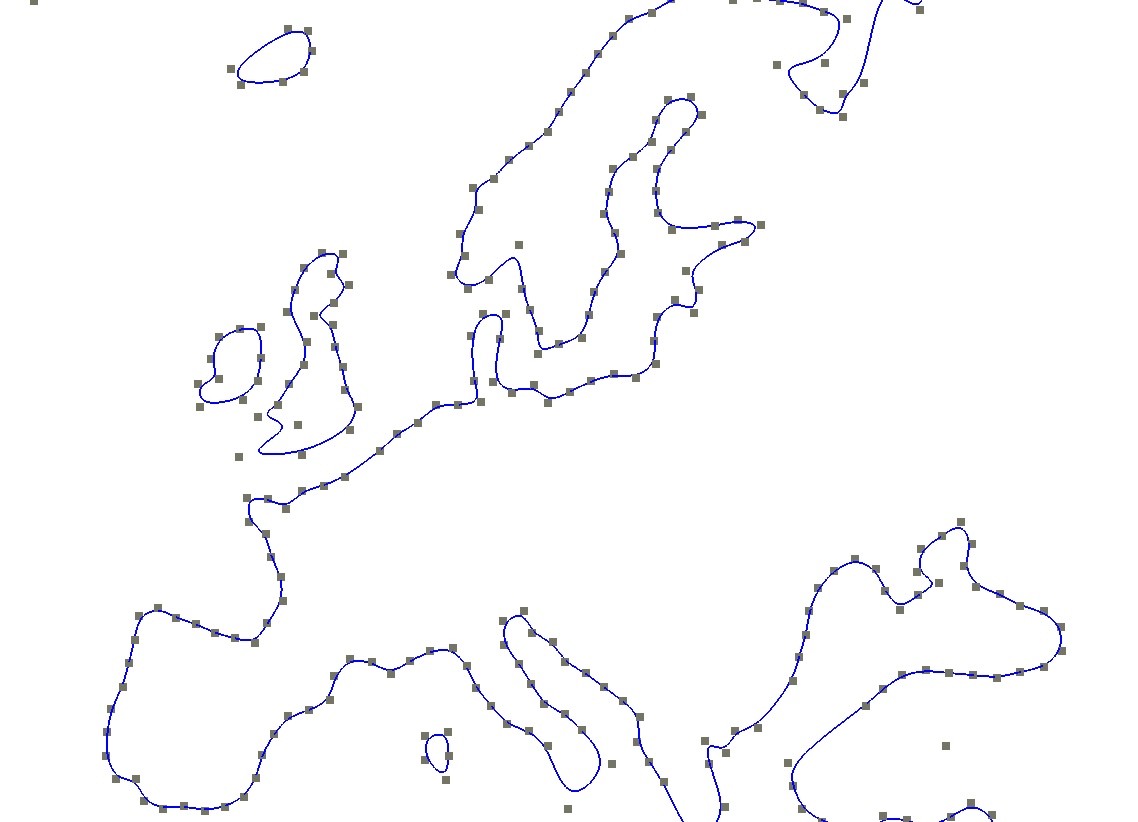
\includegraphics[width=0.7\linewidth]{./images/geometry.png}
    \centering
    \caption{Contour of Europe interpolated by B-sline}
    \label{fig:geometry}
\end{figure}

The set of all continential boundaries constitutes the "Coast", defined to be a \verb|Physical Line|. 
And the spherical surface closed by all the curves defines a \verb|Physical Surface| 
where the meshing will be performed, that's exactly the "Sea".

\subsection{Mesh Generation}
We use Gmsh to build the meshing of the ocean surface, that is the \verb|Physical Surface| we defined before. 
We expect that the mesh should be dense near the coast and sparse in the center of great ocean. 
To achieve this, we use two \verb|Field| entities to adjust the size of mesh elements at different location.

First we define an \verb|Attractor| \verb|Field| depicting the distance from a field point to the nearst
coastline. This field determines that the element size will increase when the meshing point goes further 
from the coastline.  However, we should notice that the element size can be too small thus inefficient near the boundary.
Also, generally the minimum meshing sizet should not surpass $1/6$ wavelength when running FEM to 
simulate the wave behavior.

So another \verb|Threshold Field| is applied to set a limitation on the element size.
Here we set the lower bound of element size to be 150km and maximum size to be 900km.

The mesh is generated by \verb|Frontal-Delaunay| algorithm, with 12633 nodes and 23068 elements, 
as shown in Fig.\ref{fig:mesh}.

\begin{figure}[H]
    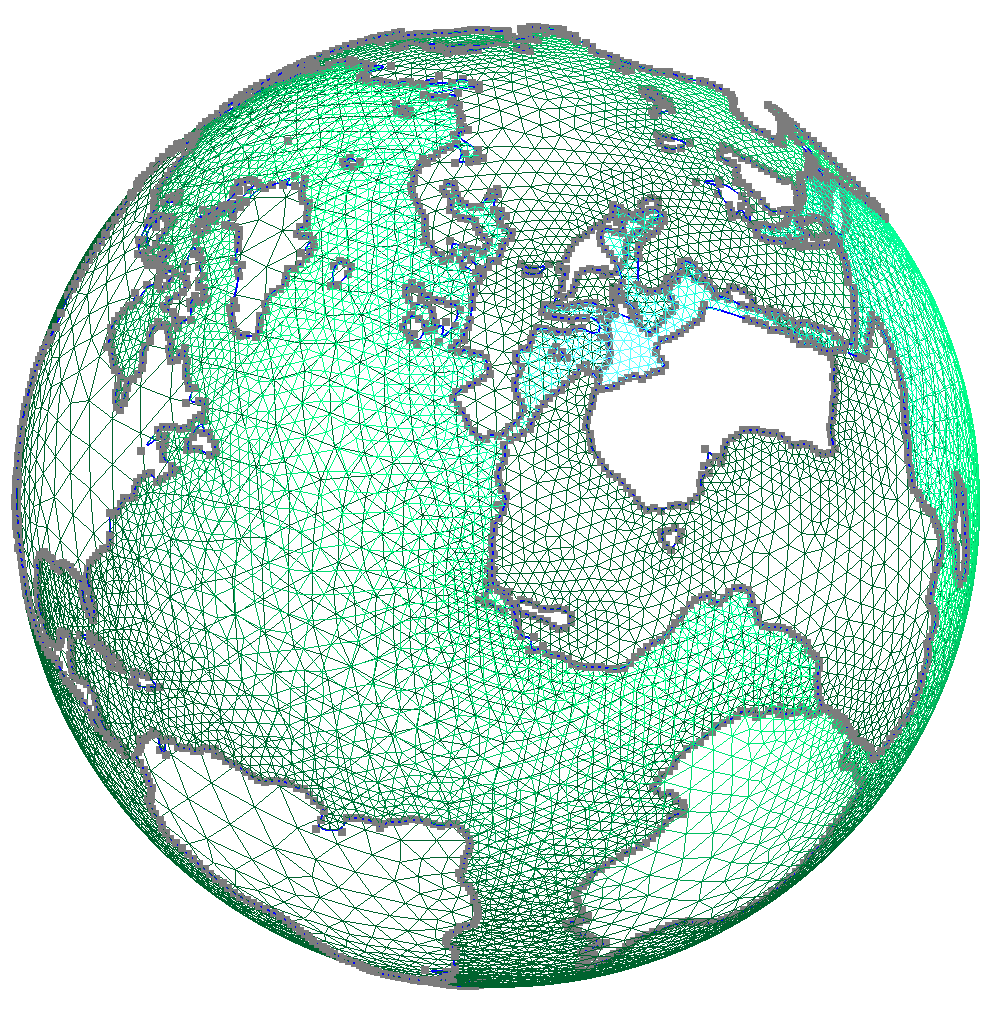
\includegraphics[width=0.83\linewidth]{./images/mesh.png}
    \centering
    \caption{World Ocean Meshing with Gmsh}
    \label{fig:mesh}
\end{figure}
    

The mesh file is exported in the \verb|.msh| format, at version 2.2.


\subsection{FEM Solution Implementation}
The algorithm is implemented in \verb|Julia|, based on the code provided in the sample.
The embeded array-based syntax and operation makes vector calculation quite convenient.
The Gmsh format data is loaded and processed using the \verb|CompScienceMeshes.jl| library.

The basic procedures implemented in the FEM are listed below
\begin{enumerate}
    \item Define the parameters (epicenter, decay rate, wavelength and so, on) and incentive functions \verb|f|. 
    \item Load meshing file and parse the data. Then the data is reorganized into structured list of elements containing local nodes. 
    This is implemented with functions \verb|read_gmsh_mesh| and \verb|skeleton| from \verb|CompScienceMeshes.jl|. 
    \item Detect boundary and interior nodes so that we can build elements matrix and vectors for different nodes.
    \item Iterate over elements and building element matrix and vectors, with \verb|elementmatrix| \verb|elementvector|.
    Also we added some necessary modifications in the module of elementary matrix to adjust for the spherical surface.
    \item Assembly the matrix and vectors in Galerkin Equation using \verb|assemblematrix| \verb|assemblevector|. The 
    mapping from local nodes index to global index, which is necessary to build the global matrix, is implemented by \verb|localtoglobal|.
    \item Solve the equation with numerical inversion of the matrix. The inversion of matrix, which is the most computation-intensive part of FEM, is implemented using 
    the build-in function of Julia. 
    \item Post-processing and visualization, using the \verb|Makie.jl| and \verb|JuliaPlot.jl|
\end{enumerate}

% \newpage
\section{Results and Discussion}
\subsection{Result Demonstration}

We start the simulation using following parameters, with an epicenter at 
North Atlantic (40.4,-43.2).
\begin{table}[h]
    \centering
    \label{tab:params_tab}
    \begin{tabular}{|c||c|c|} %|p{3cm}||p{3cm}|p{3cm}|
        % \hline
        % \multicolumn{3}{|c|}{Parameter List} \\
        \hline
        Name & Description & value\\
        \hline
        $R$ & radius of the earth & $6.371\times 10^6$ \\
        $A$   & amplitude of incentive function $f$ &  100\\
        $\sigma$   & spreading of incentive function $f$ &  $10^5$\\
        $\phi_0$ & latitude of the epicenter & $40.4\pi/180$ \\
        $\lambda_0$ & longitude of the epicenter & $-43.2\pi/180$\\
        $k$ & wavelength parameter in wave equation & $2\pi/(4\times 10^6)$\\
        \hline
    \end{tabular}
    \caption{Parameter List of Modeling}
\end{table}


With more than $10^4$ element, the solution of this FEM model can be finished in 10 sec on 
a 8-core desktop PC, which has proved the efficiency of the algorithm. 


\begin{figure*}
    \centering
    \begin{subfigure}[b]{0.475\textwidth}
        \centering
        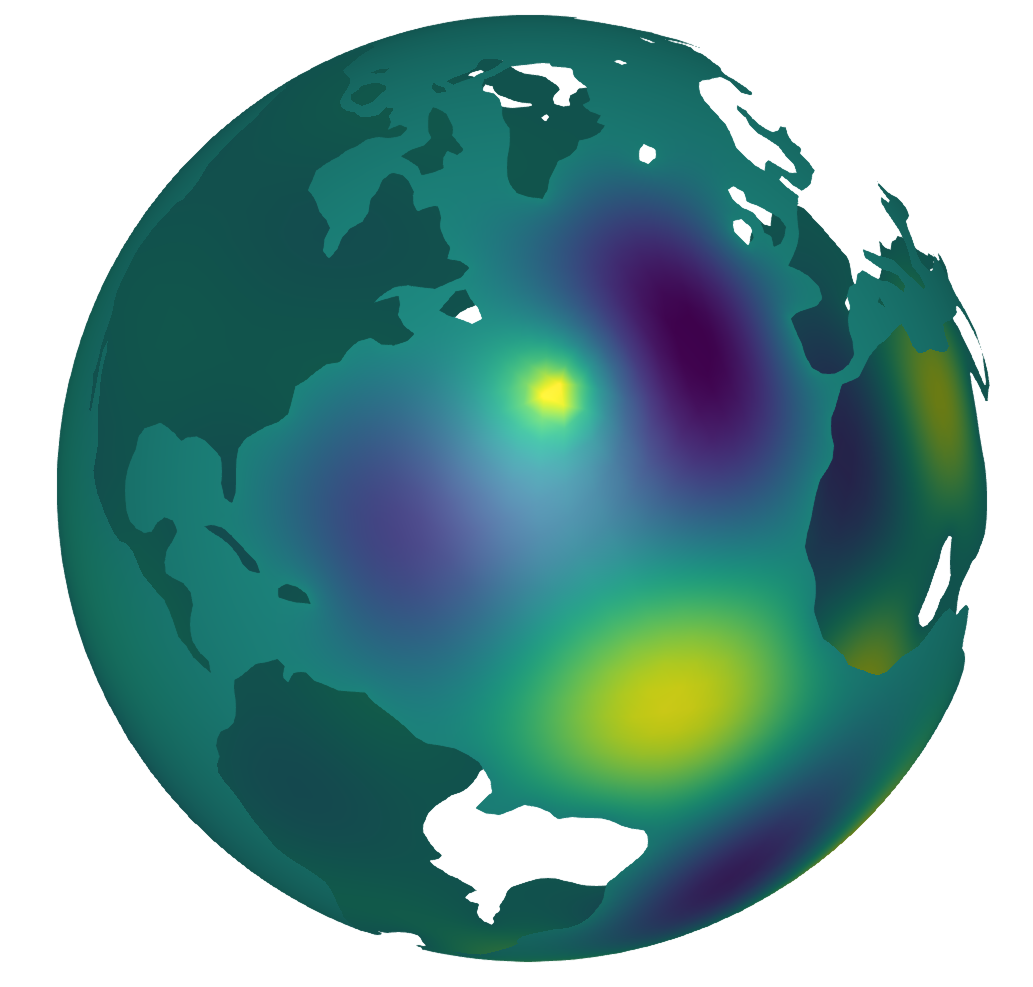
\includegraphics[width=\textwidth]{./images/shot_NAtl.png}
        \caption[]%
        {{\small North Atlantic Ocean}}    
        \label{fig:sub1}
    \end{subfigure}
    \hfill
    \begin{subfigure}[b]{0.46\textwidth}  
        \centering 
        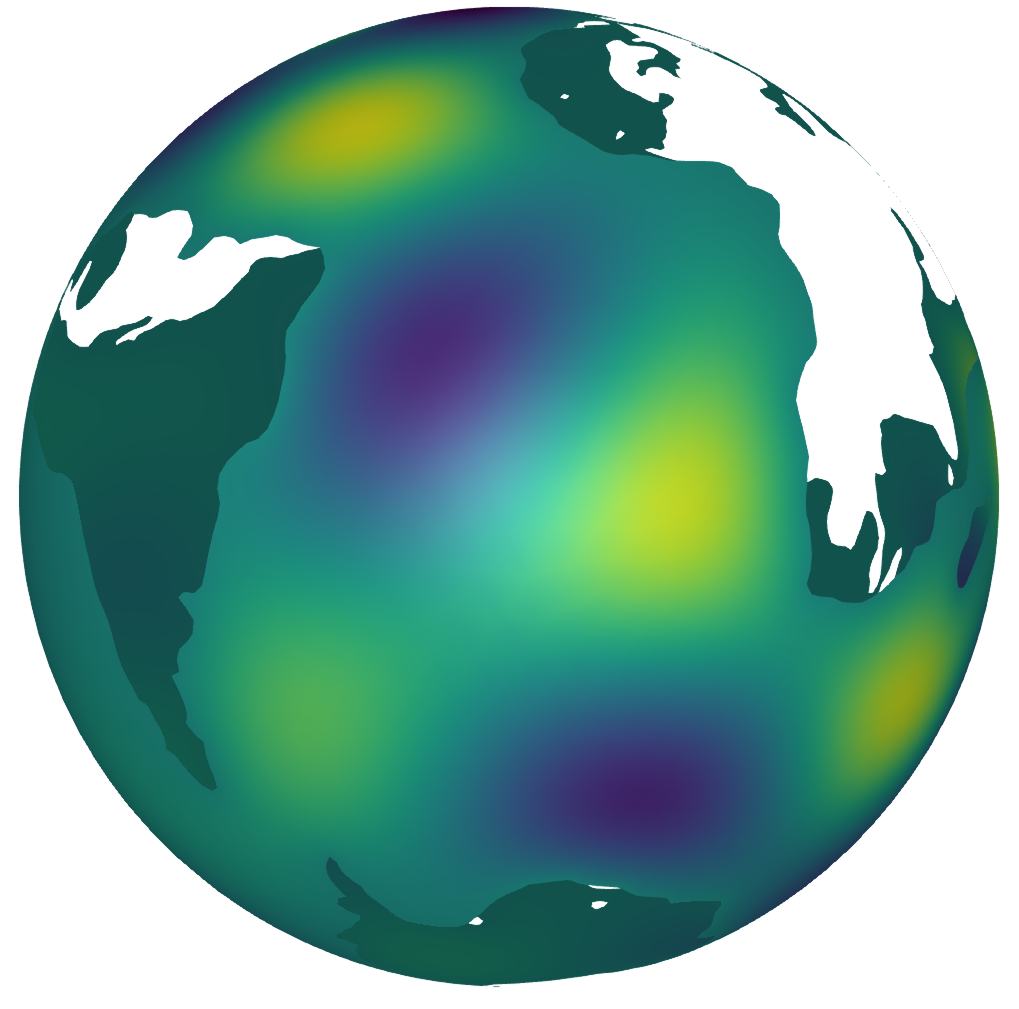
\includegraphics[width=\textwidth]{./images/shot_SAtl.png}
        \caption[]%
        {{\small South Atlantic Ocean}}    
        \label{fig:sub2}
    \end{subfigure}
    \vskip\baselineskip
    \begin{subfigure}[b]{0.475\textwidth}   
        \centering 
        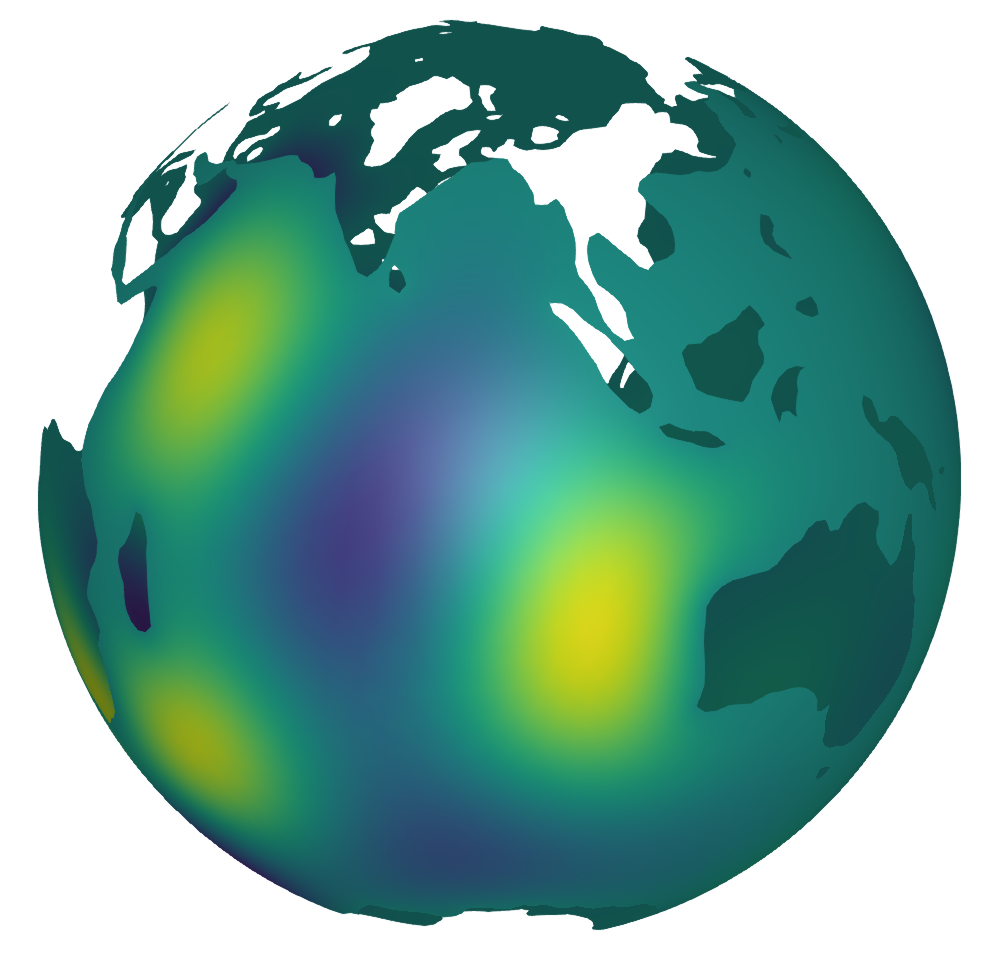
\includegraphics[width=\textwidth]{./images/shot_Ind.png}
        \caption[]%
        {{\small Indian Ocean}}    
        \label{fig:sub3}
    \end{subfigure}
    \hfill
    \begin{subfigure}[b]{0.475\textwidth}   
        \centering 
        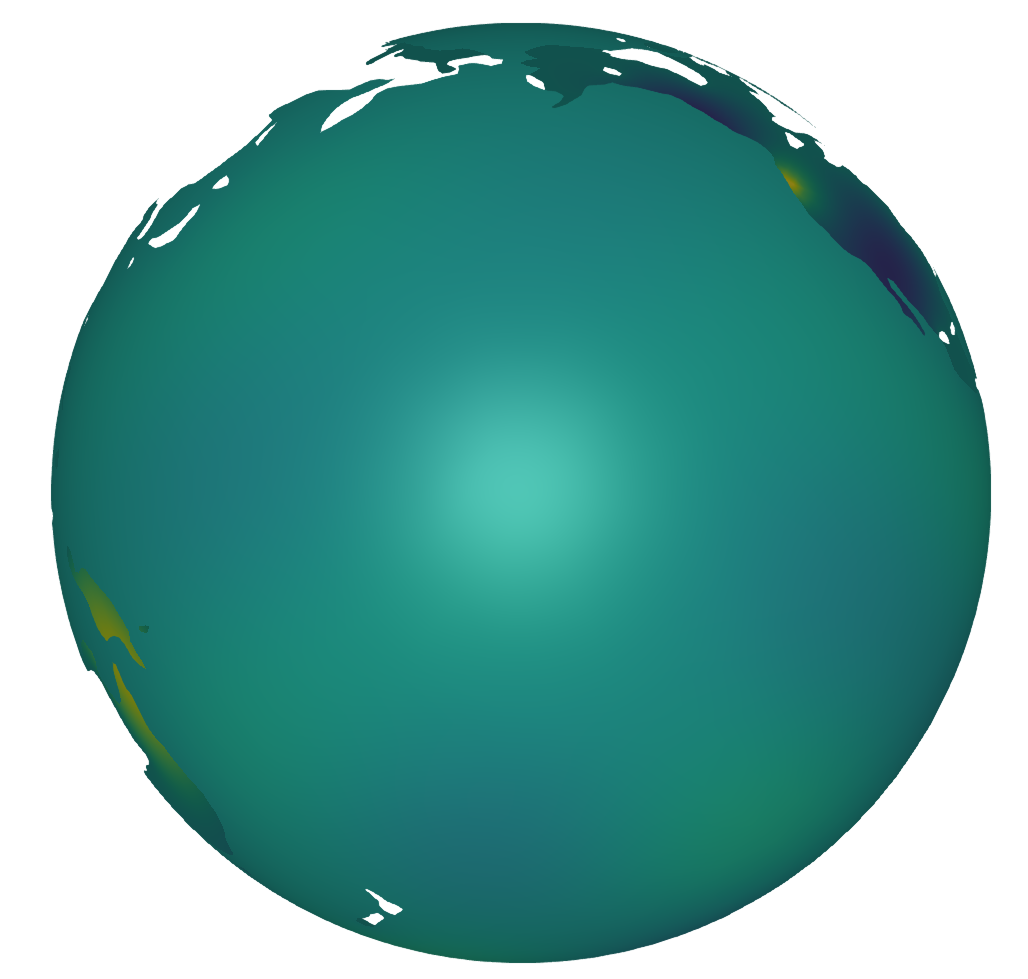
\includegraphics[width=\textwidth]{./images/shot_Pac.png}
        \caption[]%
        {{\small Pacific Ocean}}    
        \label{fig:sub4}
    \end{subfigure}
    \caption[ ]
    {\small Tsunami visualization with an epicenter on the Pacific} 
    \label{fig:result_view_2}
\end{figure*}


The result of simulation is showed in the Fig.\ref{fig:result_view}. We picked four 
different view from North Atlantic Ocean,South Atlantic Ocean, Indian Ocean, and Pacific Ocean
respectively.

Due to the input of incentive function, a bright spot 
is visuable at the epicenter of North Atlantic in \ref{fig:sub1}. The tsunami wave traveled through the
entire Atlantic Ocean and impacted the coastline of Indian Ocean.
The wavelength is set to be 4000 km thus we can see huge crests and 
troughs across the entire ocean surface.

As expected, the tsunami didn't affect the Pacific Ocean as shown in \ref{fig:sub4}. One reason is the incentive
function $f$ is set to be a Gaussian curve with $\sigma=100$ km, decaying fast with the geodesic distance to the epicenter.
Another reason is the fact that Pacific Ocean is surrounded by serveral continents, with the 
west side adjacent to Asia and Australia and east side closed by North and South America. 
With a long wavelength (4000 km), the tsunami wave can't travel through the narrow channels to Pacific,
and diffraction is also disabled.

Similar result can be acquired when we set the epiccenter on the North Pacific (15.75,154.5).
The tsunami will not travel acress the globe and impact the coastline of Atlantic and Indian Ocean.


% \begin{figure*}
%     \centering
%     \begin{subfigure}[b]{0.475\textwidth}
%         \centering
%         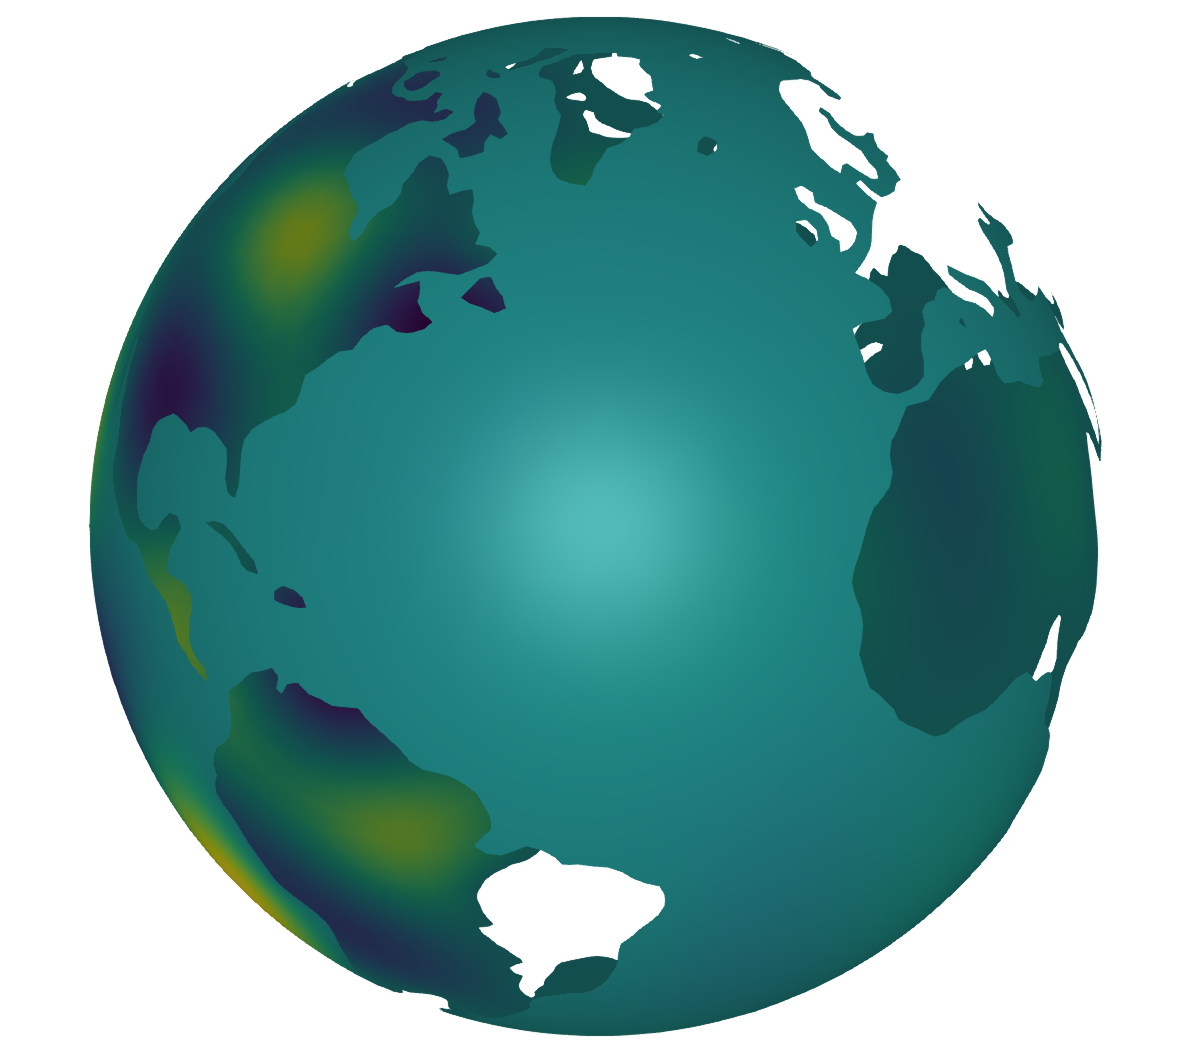
\includegraphics[width=\textwidth]{./images/shot_Atl_2.png}
%         \caption[]%
%         {{\small Atlantic Ocean}}    
%         \label{fig:sub5}
%     \end{subfigure}
%     \hfill
%     \begin{subfigure}[b]{0.46\textwidth}  
%         \centering 
%         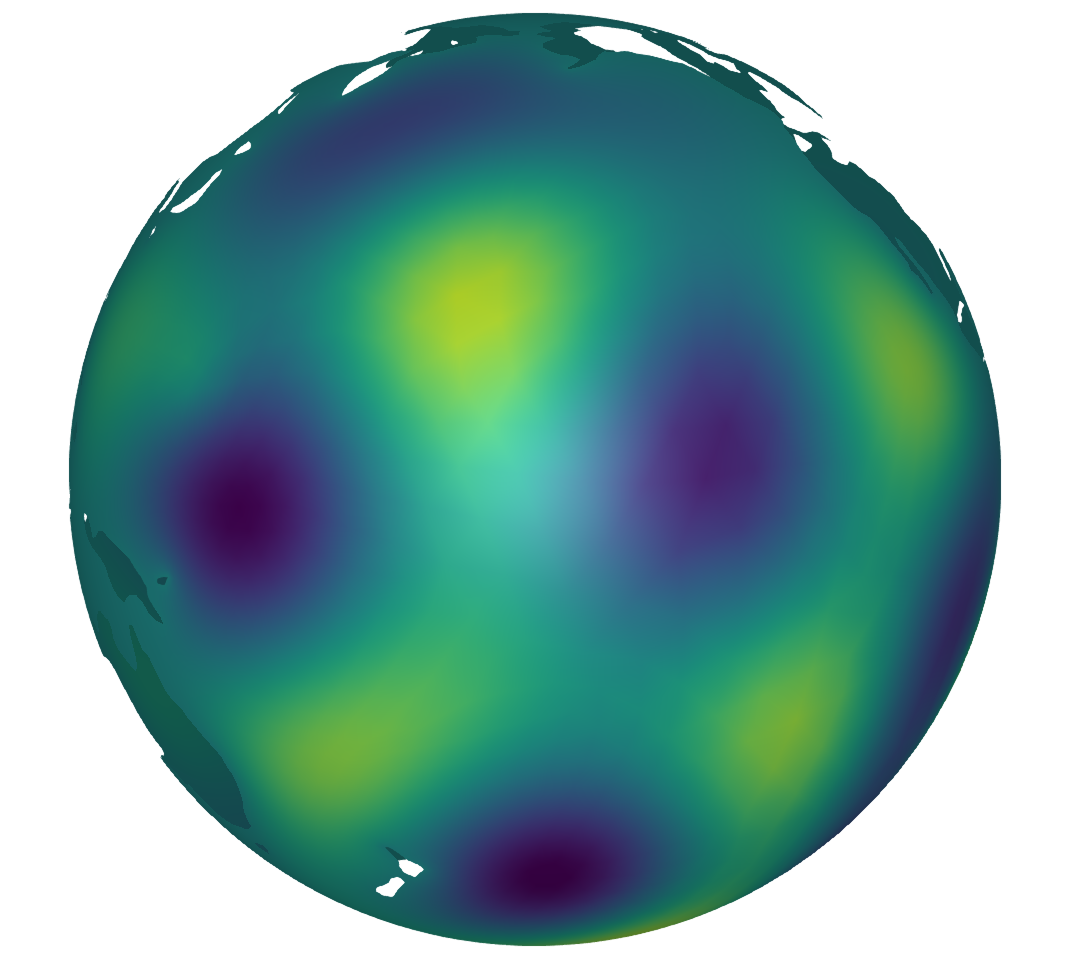
\includegraphics[width=\textwidth]{./images/shot_Pac_2.png}
%         \caption[]%
%         {{\small Pacific Ocean}}    
%         \label{fig:sub6}
%     \end{subfigure}
%     \caption[ ]
%     {\small Tsunami visualization with an epicenter on Pacific} 
%     \label{fig:result_view}
% \end{figure*}


\subsection{Comment and Improvement}
A more reasonable and conventional way to meshing the world ocean is using ocean bathymetry data\cite{amante2009etopo1}, which 
has been implemented in many oceanographical researches \cite{legrand2006high}. 
Based on bathymetry, the mesh size is supposed to be smaller in shallow ocean area and larger in deep sea region.
This can be achieved by importing a \verb|Structured Field| in \verb|Gmsh|.
Also, we can add a smaller limitations on minimum and maximum meshing size, in order to get a denser mesh.


The parameters like epicenter and wavelength can be modified, (also we need to adjust the minimum element size 
with wavelength) to explore the possible behaviors of tsunami.


Meanwhile, we must address that this model is still rough for a global tsunami. More accurate equation based on fluid dynamics
can be applied, which requires more understanding and knowledge.

%%%%%%%% EXTRA TIPS %%%%%%%%


\newpage
\bibliographystyle{ieeetr}
\bibliography{reference}


\appendix
\section{File Inventory Introduction}

\begin{itemize}
    \item \verb|./mega_tsunami.jl|:  Julia code to run the main algorithm of PDE
    \item \verb|./gshhs2geo.py|: Python script to convert GSHHS data into .geo format
    \item \verb|./mesh/gshhs/|: data folder containing data from GSHHS program
    \item \verb|./mesh/world.geo|: Gmsh .geo format file that contains the model geometry
    \item \verb|./mesh/world.msh|: Gmsh .msh format file that contains mesing of the model
\end{itemize}


\end{document}